% !TEX root =  ../supplementary.tex

\section{Non-compliance in PRIAS}
The PRIAS schedule for biopsies is: one biopsy each at year one, year four, year seven and year ten (and every five years thereafter) after induction in AS. If at any time point a patient has PSA-DT less than 10 years, then biopsies are conducted annually, where, PSA-DT is measured as the inverse of the slope of regression line through the base two logarithm of observed PSA levels. However, it has been observed by \citet{bokhorst2015compliance} that patients/doctors do not always comply with this biopsy schedule. Some of the reasons given by patients/doctors for non-compliance are: `patient does not want biopsy', `PSA stable', `complications on last biopsy' and `no signs of disease progression on previous biopsy'. Such non-compliance can lead to delays in detection of prostate cancer progression. To elucidate the issue of non-compliance in PRIAS, we show in Web Figure \ref{web_fig : non_compliance} a histogram of the repeat biopsies conducted for the PRIAS patients who never obtained GR (4560 out 5267 patients). It can be seen that the compliance for the first repeat biopsy around year one is much higher than the same at later years.

\begin{figure}
\centerline{
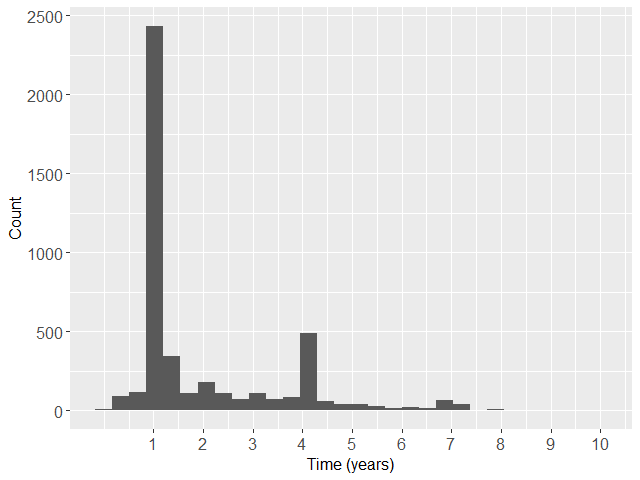
\includegraphics[width=\columnwidth]{images/non_compliance.png}
}
\caption{Histogram of repeat biopsies conducted for the 4560 out of 5267 PRIAS patients who did not obtain GR.}
\label{web_fig : non_compliance}
\end{figure}